\documentclass{beamer}

% Theme configuration
\usetheme{Madrid}
\usecolortheme{dolphin}

% Required packages
\usepackage[utf8]{inputenc}
\usepackage[T1]{fontenc}
\usepackage[english]{babel}
\usepackage{graphicx}
\usepackage{booktabs}
\usepackage{amsmath}
\usepackage{hyperref}
\usepackage{xcolor}
\usepackage{listings}

% Custom colors
\definecolor{primary}{RGB}{0,102,204}
\definecolor{secondary}{RGB}{102,102,153}
\definecolor{accent}{RGB}{204,0,0}
\definecolor{codegray}{rgb}{0.5,0.5,0.5}
\definecolor{codepurple}{rgb}{0.58,0,0.82}
\definecolor{codeblue}{rgb}{0,0,0.9}
\definecolor{codegreen}{rgb}{0.1,0.6,0.1}

% Code listing style
\lstdefinestyle{codestyle}{
    basicstyle=\ttfamily\footnotesize,
    numbers=left,
    numberstyle=\tiny\color{codegray},
    stepnumber=1,
    numbersep=5pt,
    backgroundcolor=\color{white!95!black},
    showspaces=false,
    showstringspaces=false,
    showtabs=false,
    frame=tb,
    tabsize=2,
    captionpos=b,
    breaklines=true,
    breakatwhitespace=false,
    stringstyle=\color{codepurple},
    commentstyle=\color{codegreen},
    keywordstyle=\color{codeblue}
}

% Image path configuration
\graphicspath{{week_1_img/}{week_2_img/}{week_3_img/}{week_4_img/}{images/}{./}{/home/ziko/Documents/web_presentation/images/}}

% Title information
\title[LearnExpert Platform]{Design and Development of an E-learning Platform}
\subtitle{Internship Report - IAAI Academy}
\author[Zakaria el Khaldi]{Zakaria el Khaldi}
\institute[BTS Al-Kendi]{Al-Kendi BTS Center, Casablanca}
\date{June 2025}
\logo{\includegraphics[height=1cm]{LOGO_IAAI.png}}

\begin{document}

\frame{\titlepage}

\begin{frame}
\frametitle{Presentation Outline}
\tableofcontents
\end{frame}

% 1. Introduction (2 min)
\section{Introduction}

\begin{frame}
\frametitle{Project Overview}
\begin{itemize}
    \item \textbf{Context}: 4-week internship at IAAI Academy
    \item \textbf{Project}: LearnExpert e-learning platform
    \item \textbf{Objective}: Development of an interactive learning solution for programming and web technologies
\end{itemize}
\begin{center}
    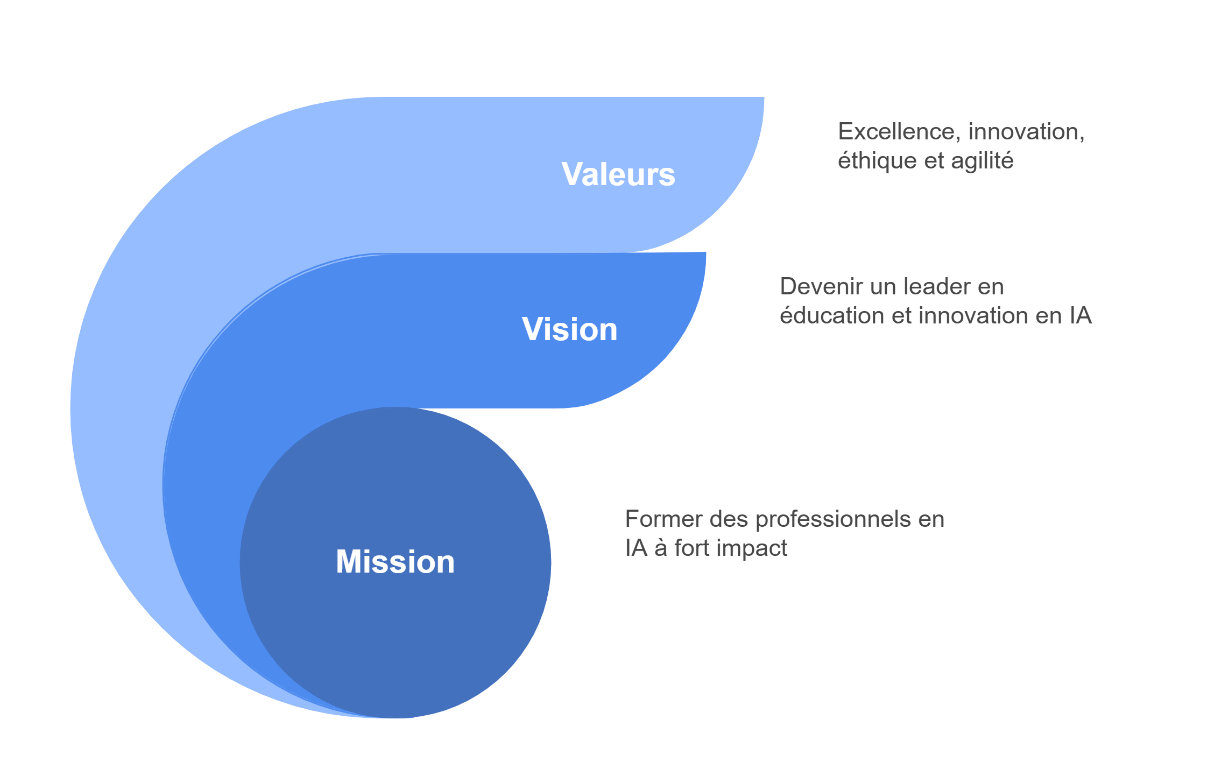
\includegraphics[width=0.5\textwidth]{images/mession.png}
\end{center}
\end{frame}

\begin{frame}
\frametitle{Challenges and Objectives}
\begin{columns}
\column{0.5\textwidth}
\textbf{Identified challenges:}
\begin{itemize}
    \item Generic content in existing platforms
    \item Lack of interactivity for programming learning
    \item Fragmentation of educational resources
    \item Absence of personalization
\end{itemize}

\column{0.5\textwidth}
\textbf{Project objectives:}
\begin{itemize}
    \item Practice-centered approach
    \item AI-powered personalization
    \item Structured content integration
    \item Scalable architecture
    \item Engaging user experience
\end{itemize}
\end{columns}
\end{frame}

% 2. Methodology (2 min)
\section{Methodology}

\begin{frame}
\frametitle{Development Approach}
\begin{columns}
\column{0.5\textwidth}
\textbf{Adopted methodology:}
\begin{itemize}
    \item Adapted waterfall approach
    \item Structured phases
    \item Iterative reviews
    \item Incremental development
\end{itemize}

\column{0.5\textwidth}
\textbf{Modeling tools:}
\begin{itemize}
    \item UML (Unified Modeling Language)
    \item Use case diagrams
    \item Sequence diagrams
    \item Class diagrams
    \item Data models
\end{itemize}
\end{columns}
\end{frame}

\begin{frame}
\frametitle{Project Planning}
\begin{itemize}
    \item \textbf{Project timeline}: Four-week development period
    \item \textbf{Phase organization}:
    \begin{itemize}
        \item Week 1: Design and architecture
        \item Week 2: Frontend foundation and landing page
        \item Week 3: Learning interface and dashboard
        \item Week 4: Interactive features and refinements
    \end{itemize}
    \item \textbf{Critical path management}: Focus on essential components first
\end{itemize}
\begin{center}
    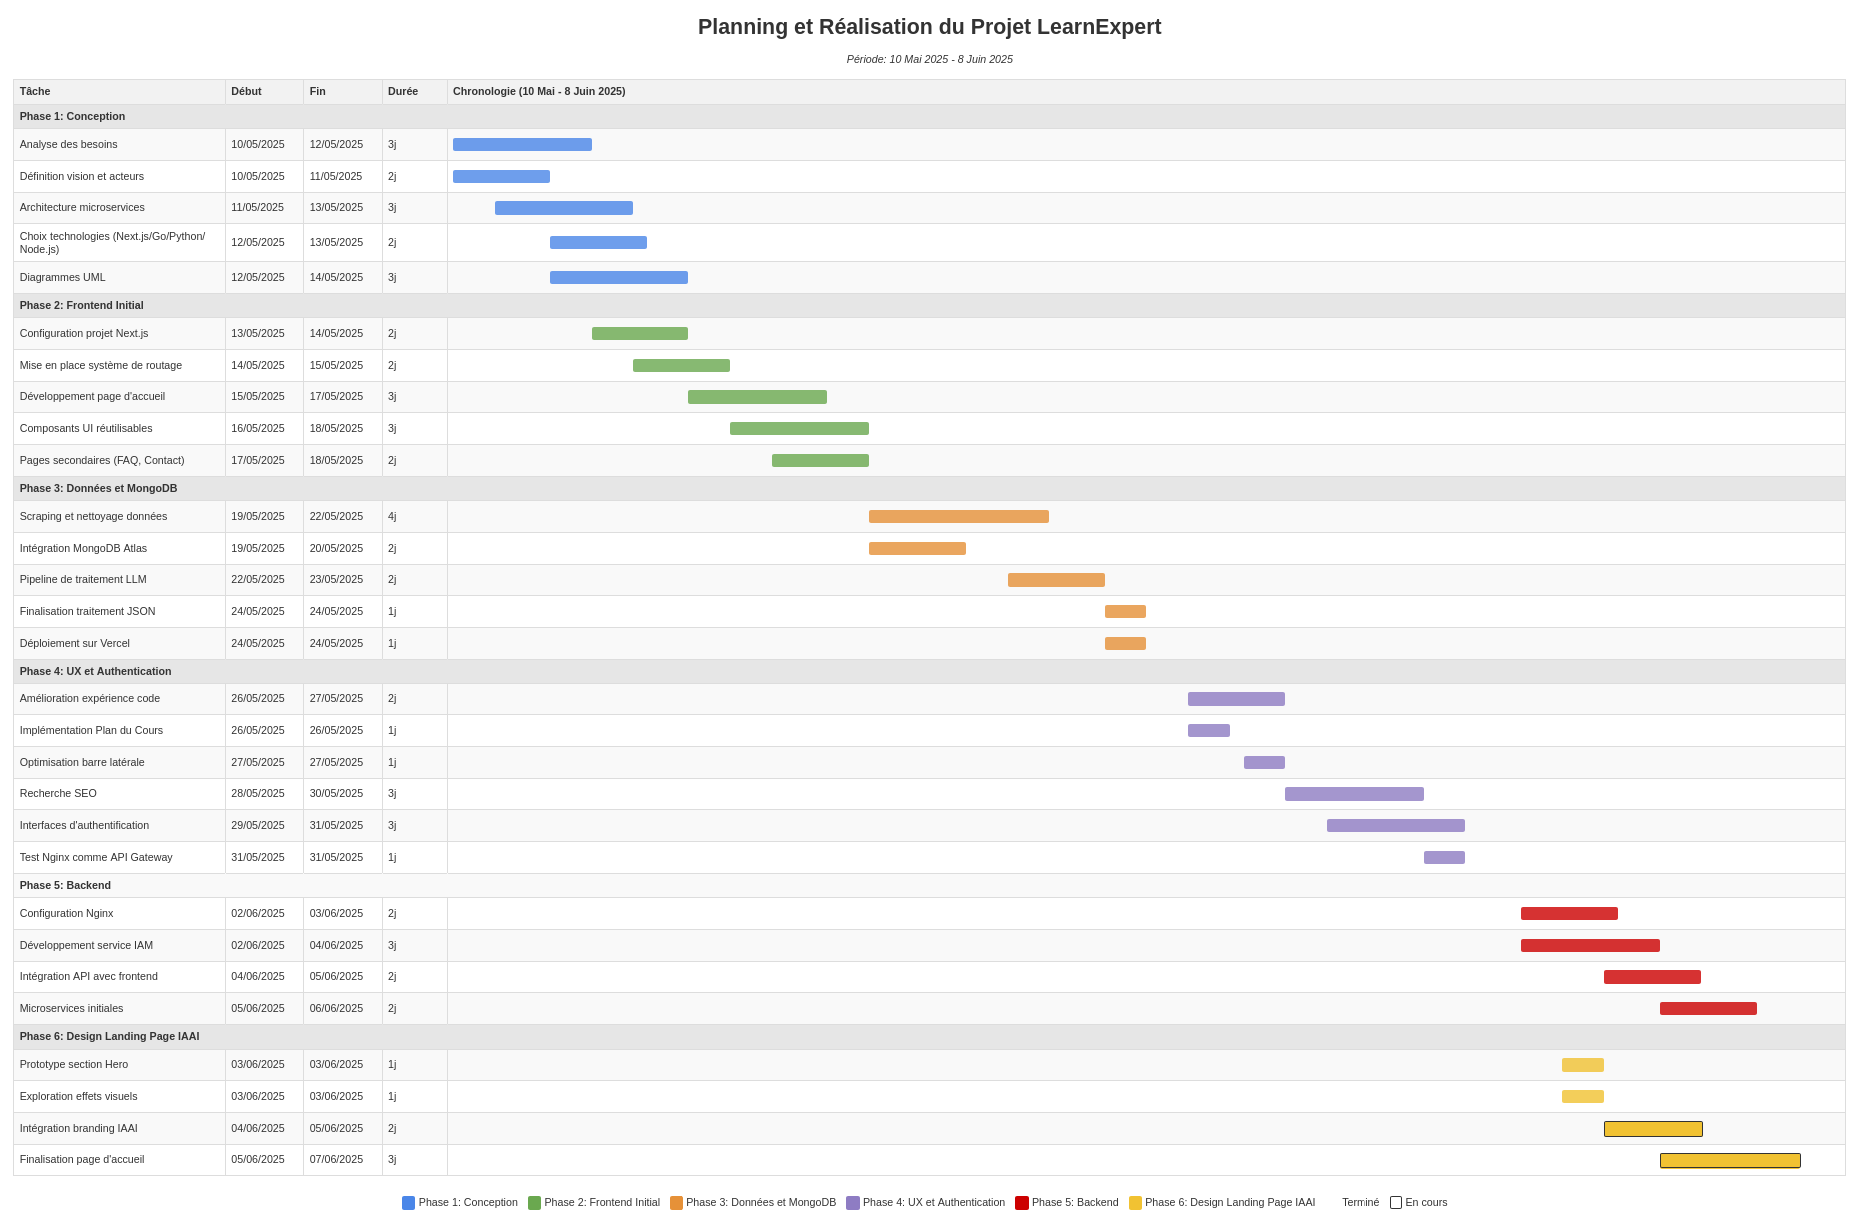
\includegraphics[width=0.95\textwidth,height=5cm,keepaspectratio]{Screenshot 2025-06-08 at 20-35-06 Planning du Projet LearnExpert - Diagramme de Gantt.png}
\end{center}
\end{frame}

% 3. System Architecture (4 min)
\section{System Architecture}

\begin{frame}
\frametitle{Architecture Overview}
\begin{center}
    \includegraphics[width=0.9\textwidth,height=6cm,keepaspectratio]{architecture_diagram.png}
\end{center}
\end{frame}

\begin{frame}
\frametitle{Microservices Architecture}
\begin{columns}
\column{0.5\textwidth}
\textbf{Benefits of microservices:}
\begin{itemize}
    \item Independent service scalability
    \item Improved maintainability
    \item Enhanced resilience
    \item Technological flexibility
\end{itemize}

\column{0.5\textwidth}
\textbf{Core services:}
\begin{itemize}
    \item IAM Service
    \item Content Service
    \item Billing Service
    \item Certification Service
    \item Analytics Service
    \item Notification Service
\end{itemize}
\end{columns}

\vspace{0.3cm}
\begin{center}
    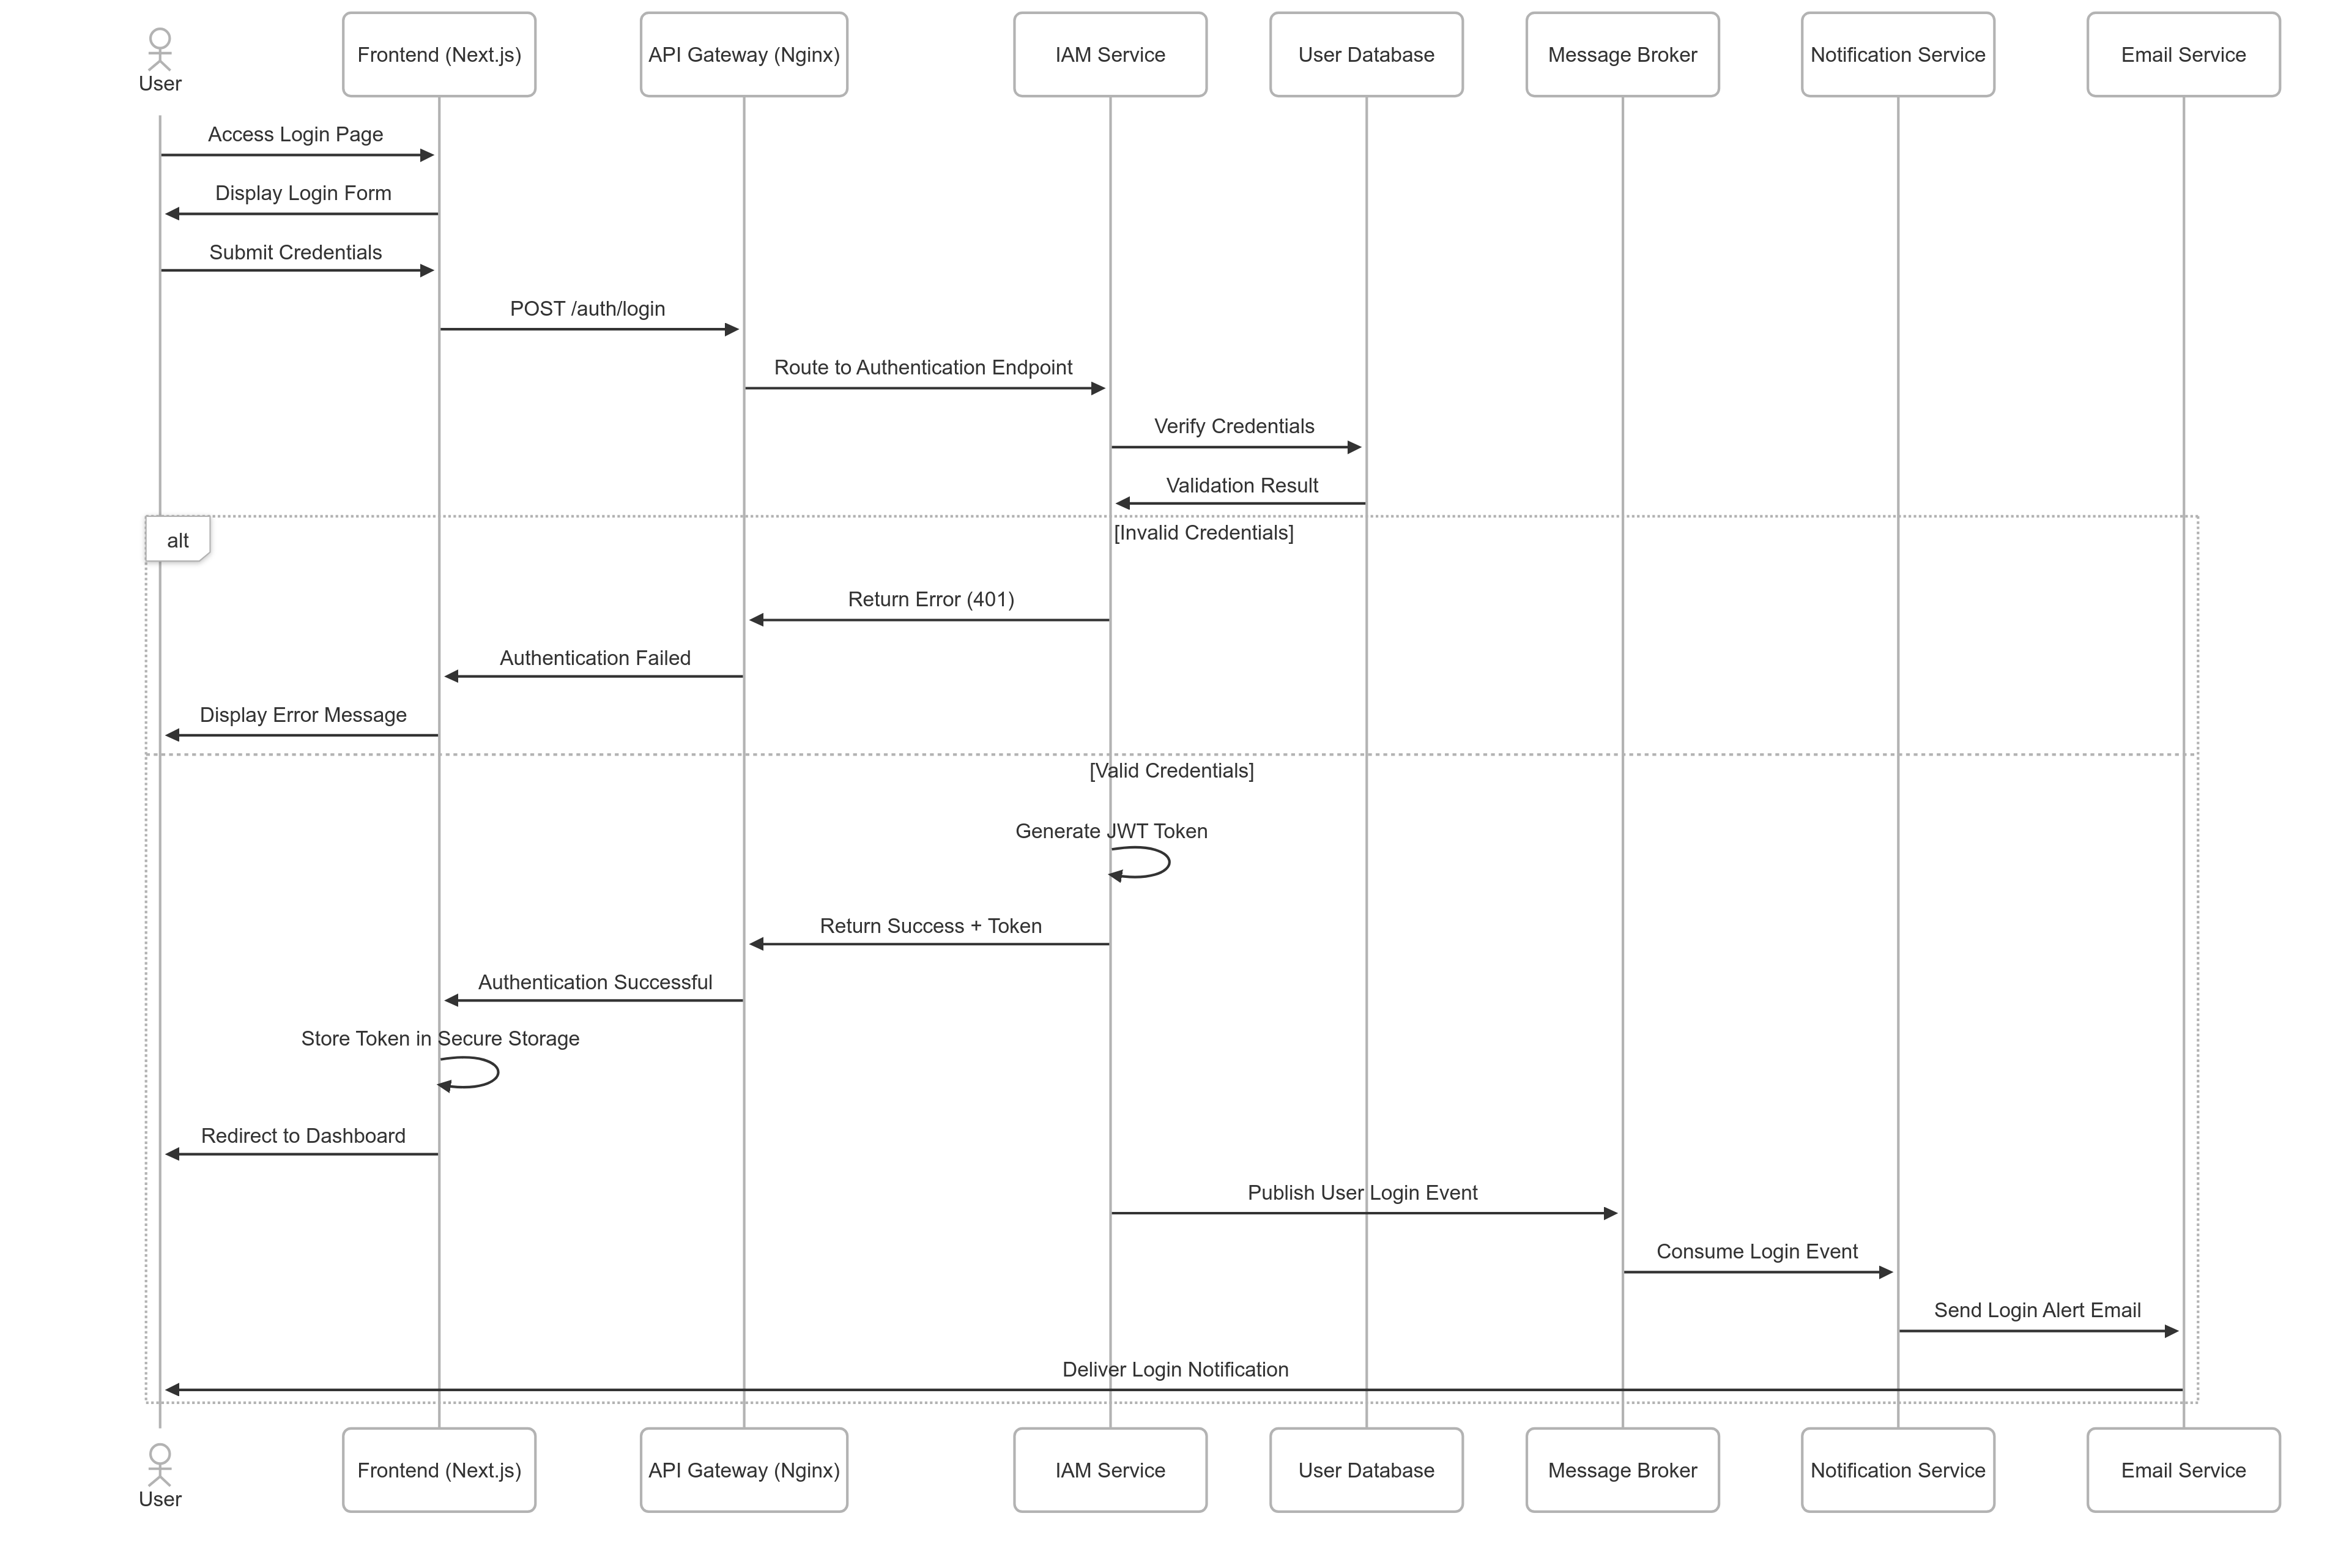
\includegraphics[width=0.8\textwidth,height=3.5cm,keepaspectratio]{Editor _ Mermaid Chart-2025-06-06-214630.png}
\end{center}
\end{frame}

\begin{frame}
\frametitle{Frontend Technologies}
\begin{columns}
\column{0.5\textwidth}
\textbf{Framework and languages:}
\begin{itemize}
    \item Next.js (React)
    \item TypeScript
    \item Tailwind CSS
    \item Framer Motion
\end{itemize}

\column{0.5\textwidth}
\textbf{Specialized tools:}
\begin{itemize}
    \item Monaco Editor (code editor)
    \item React Hook Form (form management)
    \item Radix UI (accessible components)
\end{itemize}
\end{columns}
\begin{center}
    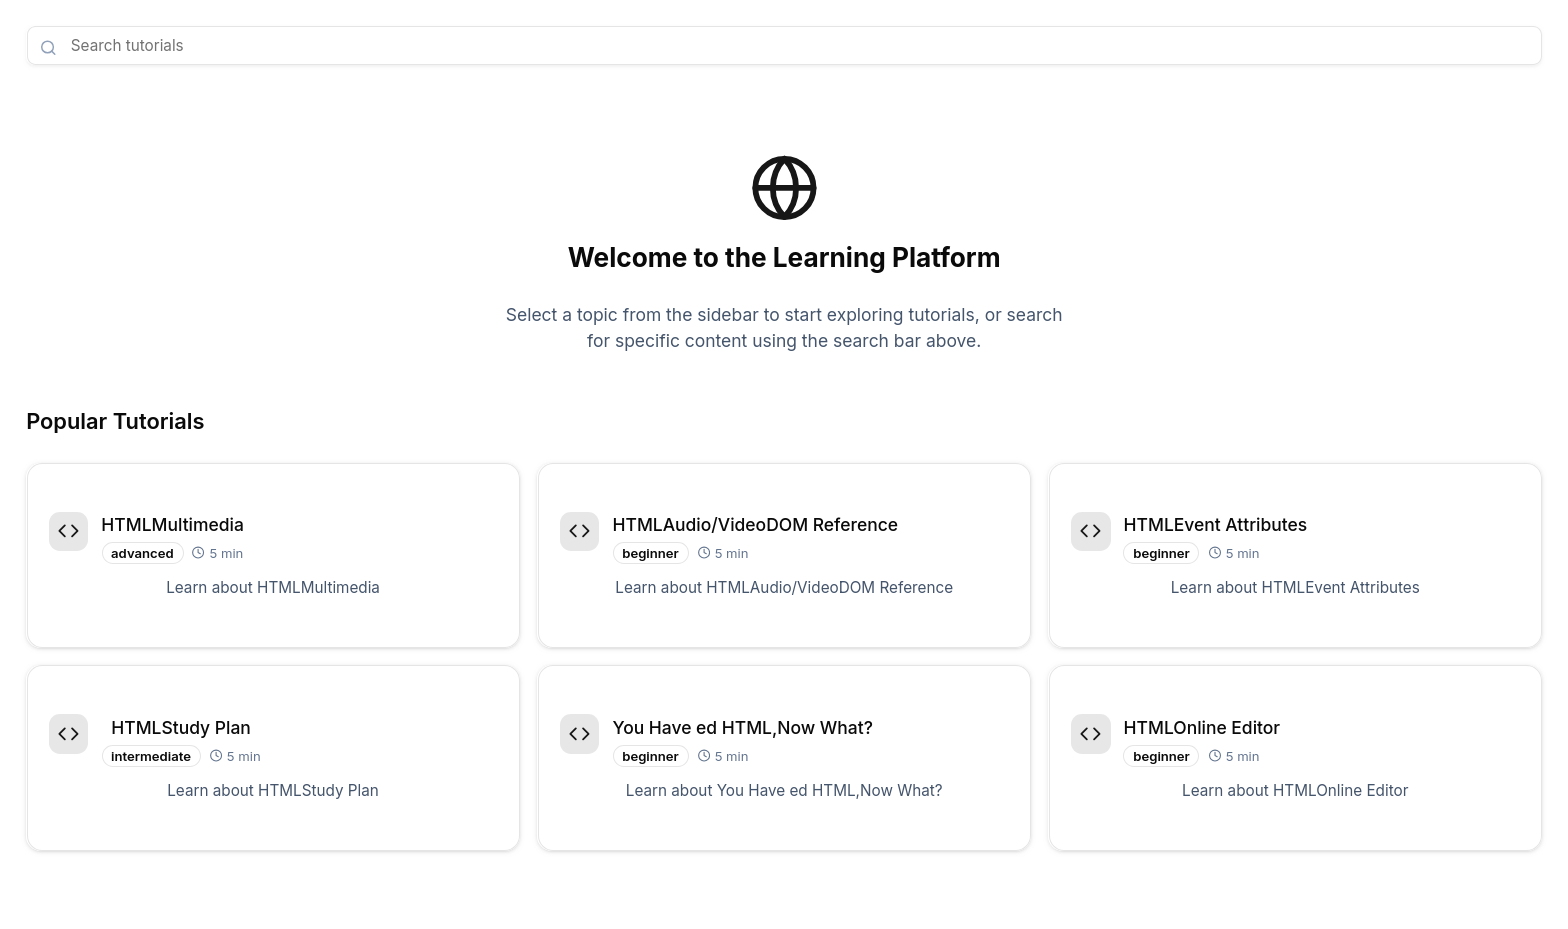
\includegraphics[width=0.5\textwidth]{week_3_img/accueil.png}
\end{center}
\end{frame}

\begin{frame}
\frametitle{Backend Technologies}
\begin{columns}
\column{0.5\textwidth}
\textbf{Languages and frameworks:}
\begin{itemize}
    \item Node.js with Express
    \item Python with FastAPI
    \item Go (for critical services)
\end{itemize}

\column{0.5\textwidth}
\textbf{Infrastructure:}
\begin{itemize}
    \item Nginx (API Gateway)
    \item MongoDB (unstructured data)
    \item PostgreSQL/Supabase (relational data)
    \item Docker (containerization)
    \item Apache Kafka (event-driven communication)
\end{itemize}
\end{columns}
\end{frame}

\begin{frame}
\frametitle{Database Design}
\begin{columns}
\column{0.48\textwidth}
\textbf{IAM Model:}
\begin{center}
    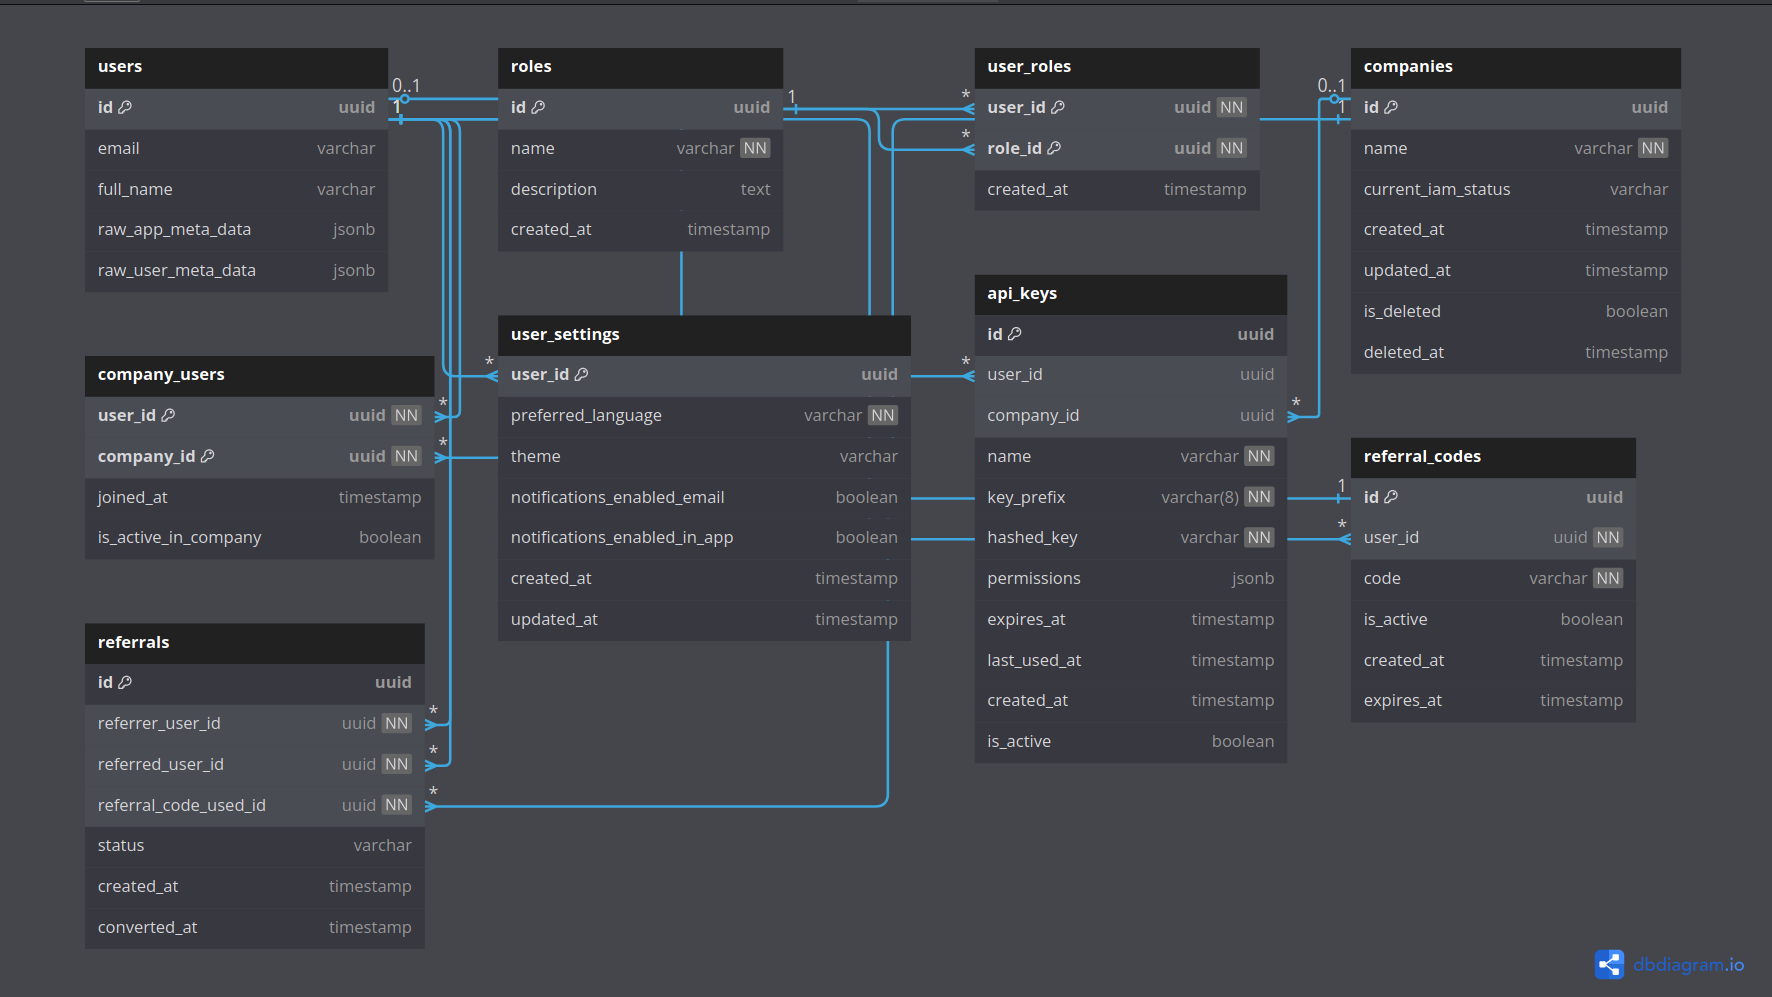
\includegraphics[width=\textwidth,height=5cm,keepaspectratio]{week_1_img/services_db_screanshots/Screenshot 2025-06-06 at 15-08-36 IAM_Service.pdf.png}
\end{center}

\column{0.48\textwidth}
\textbf{Content Model:}
\begin{center}
    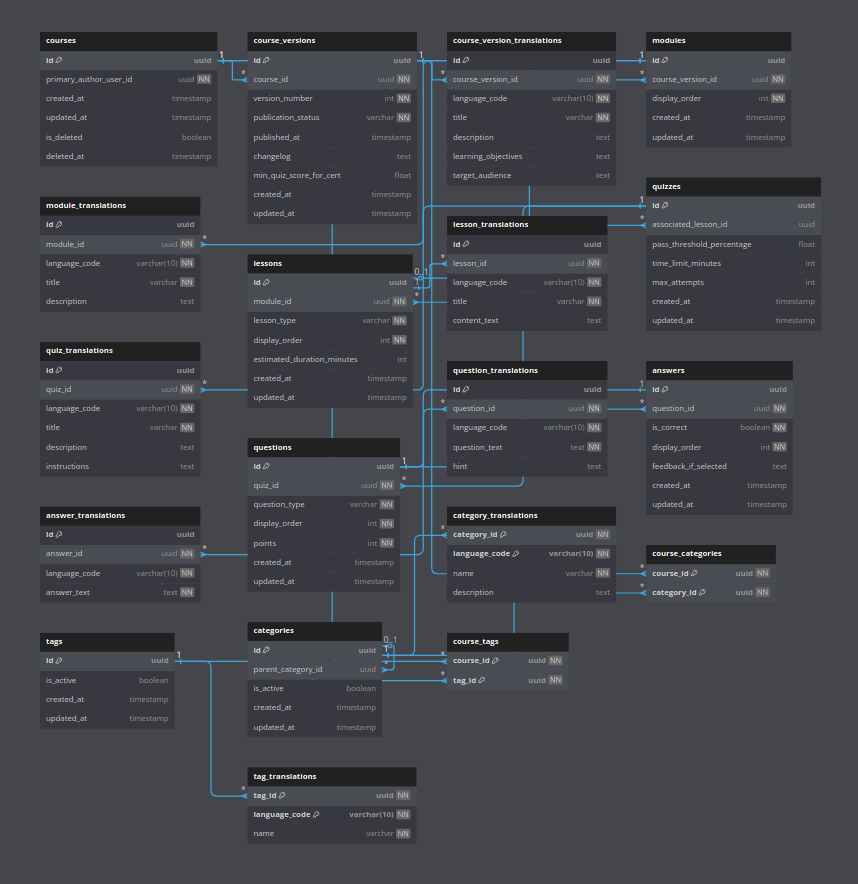
\includegraphics[width=\textwidth,height=5cm,keepaspectratio]{week_1_img/services_db_screanshots/Screenshot 2025-06-06 at 15-07-51 Content_Service.pdf.png}
\end{center}
\end{columns}
\end{frame}

% 4. Key Features & Functionality (4 min)
\section{Key Features \& Functionality}

\begin{frame}
\frametitle{User Management System}
\begin{itemize}
    \item \textbf{Multi-level authentication}
    \begin{itemize}
        \item Secure registration and login
        \item Email verification
        \item Password recovery
    \end{itemize}
    \item \textbf{Role management}
    \begin{itemize}
        \item Individual learner
        \item Company employee
        \item Company administrator
        \item Content creator
        \item Consultant
        \item Support agent
        \item Platform administrator
    \end{itemize}
    \item \textbf{Profile customization}
    \item \textbf{Privacy and notification settings}
\end{itemize}
\end{frame}

\begin{frame}
\frametitle{Course Management}
\begin{columns}
\column{0.48\textwidth}
\textbf{Content organization:}
\begin{itemize}
    \item Hierarchical structure
    \item Multi-format support (text, code, video)
    \item Advanced metadata
    \item Versioning
\end{itemize}

\column{0.48\textwidth}
\textbf{Learning interface:}
\begin{itemize}
    \item Structured theoretical content
    \item Integrated practical exercises
    \item Intuitive navigation
    \item Dark/light mode
\end{itemize}
\end{columns}

\vspace{0.3cm}
\begin{center}
    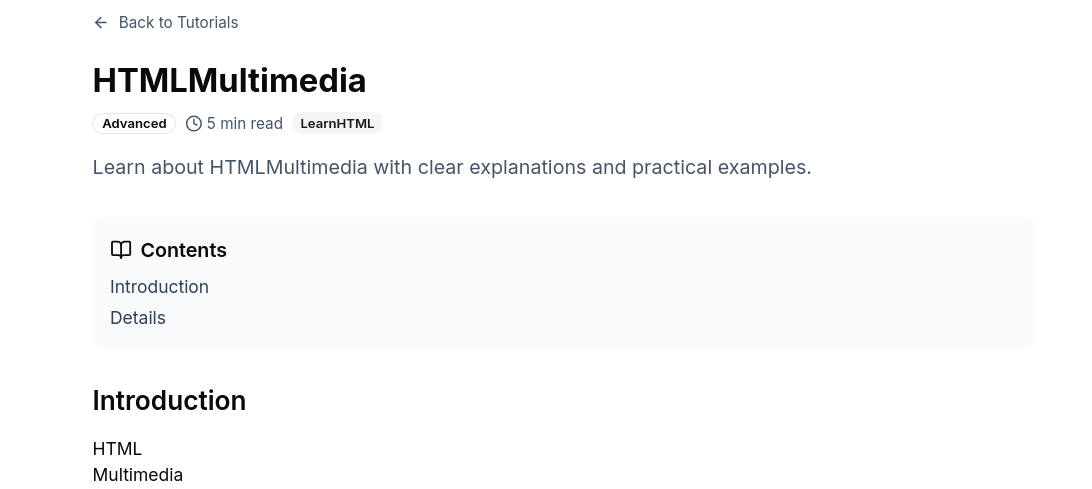
\includegraphics[width=0.65\textwidth,height=4cm,keepaspectratio]{week_3_img/part1.png}
\end{center}
\end{frame}

\begin{frame}
\frametitle{Learning Paths}
\begin{columns}
\column{0.55\textwidth}
\textbf{Specialized thematic paths:}
\begin{itemize}
    \item Artificial Intelligence
    \item Cybersecurity
    \item IT Skills
    \item Technical interview preparation
\end{itemize}
\textbf{Features:}
\begin{itemize}
    \item Intelligent personalization
    \item Structured progression
    \item Adaptive dashboard
\end{itemize}

\column{0.42\textwidth}
\begin{center}
    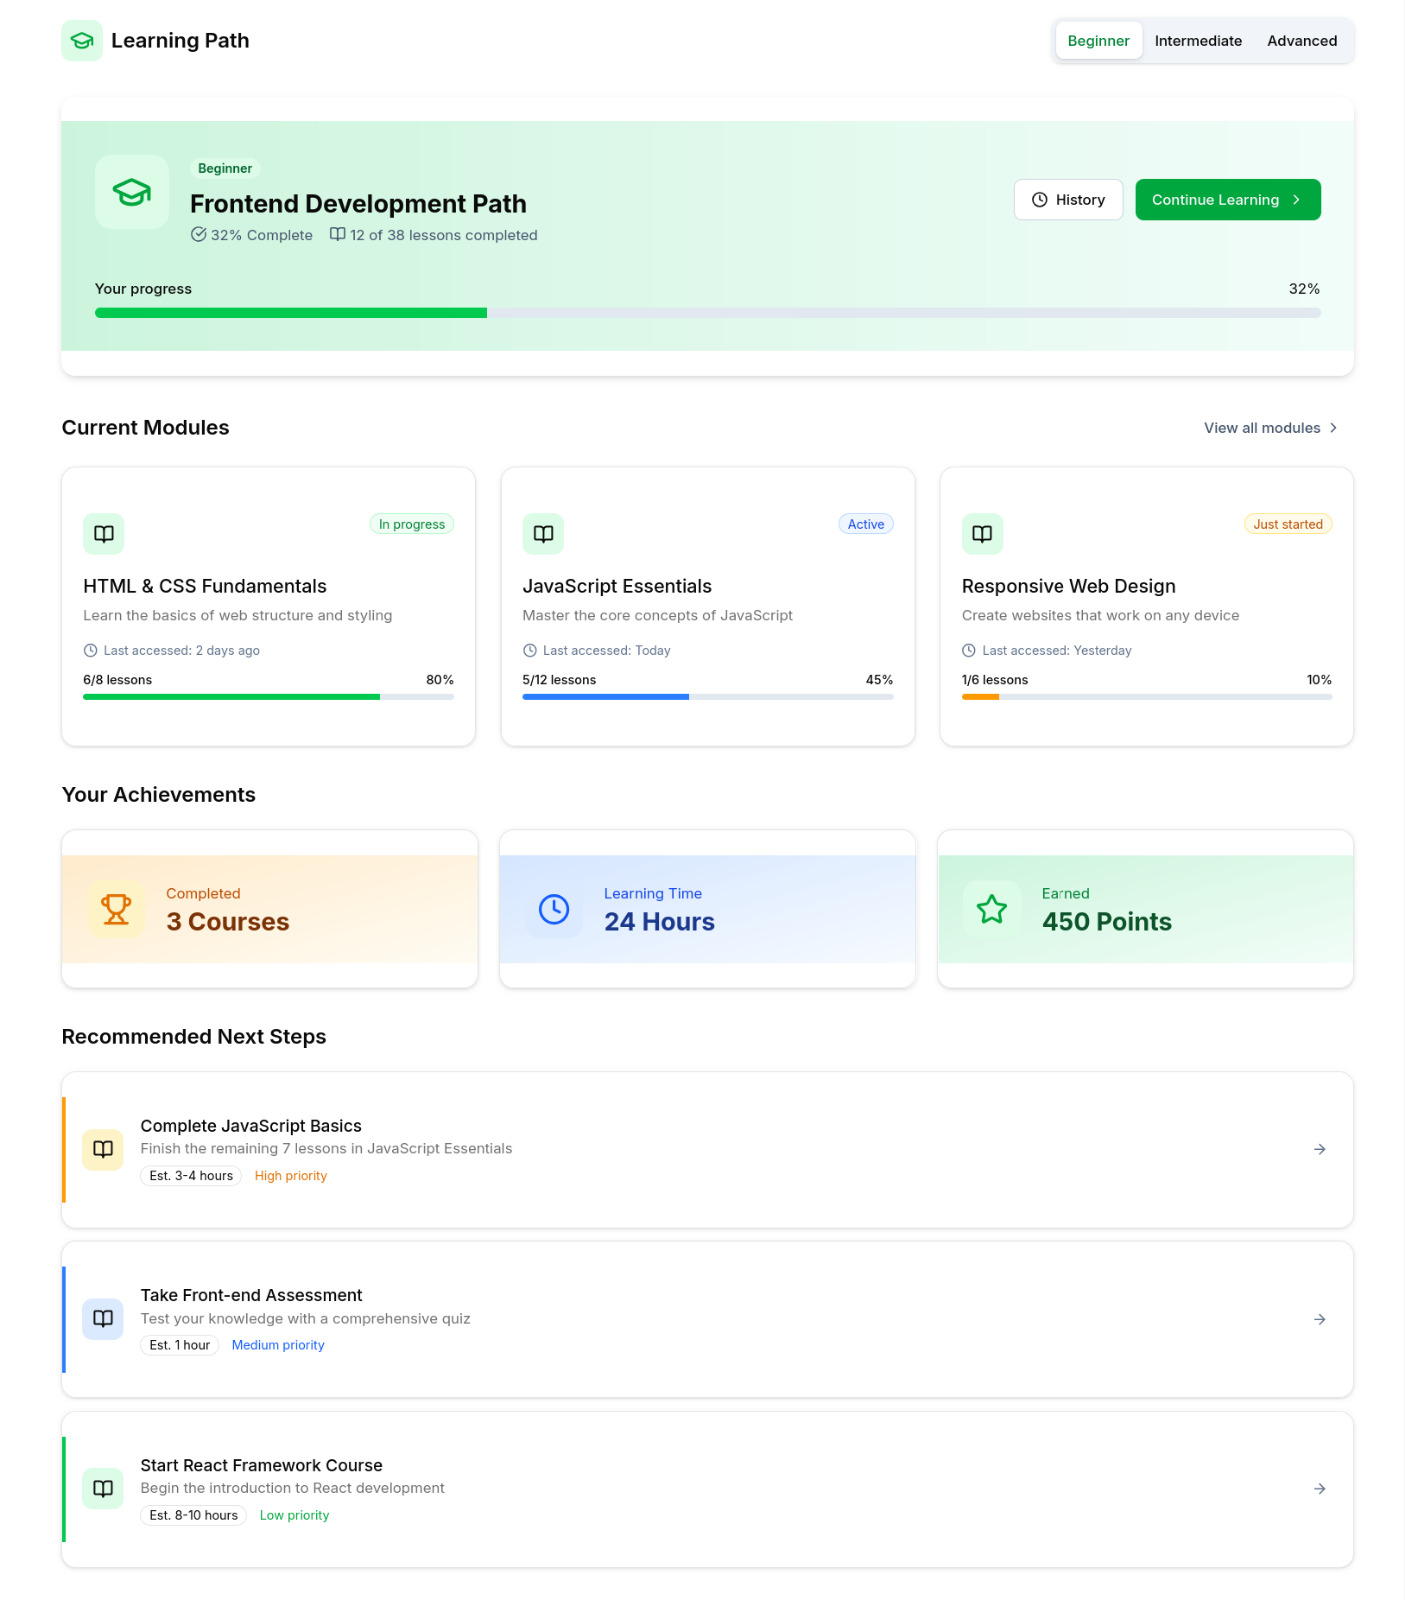
\includegraphics[width=\textwidth,height=5cm,keepaspectratio]{old-reports/week_4_img/learnpath.jpeg}
\end{center}
\end{columns}
\end{frame}

\begin{frame}
\frametitle{Assessment and Certification}
\begin{columns}
\column{0.5\textwidth}
\textbf{Evaluation systems:}
\begin{itemize}
    \item Interactive quizzes
    \item Code exercises with verification
    \item Personalized feedback
    \item Practical projects
\end{itemize}

\column{0.46\textwidth}
\begin{center}
    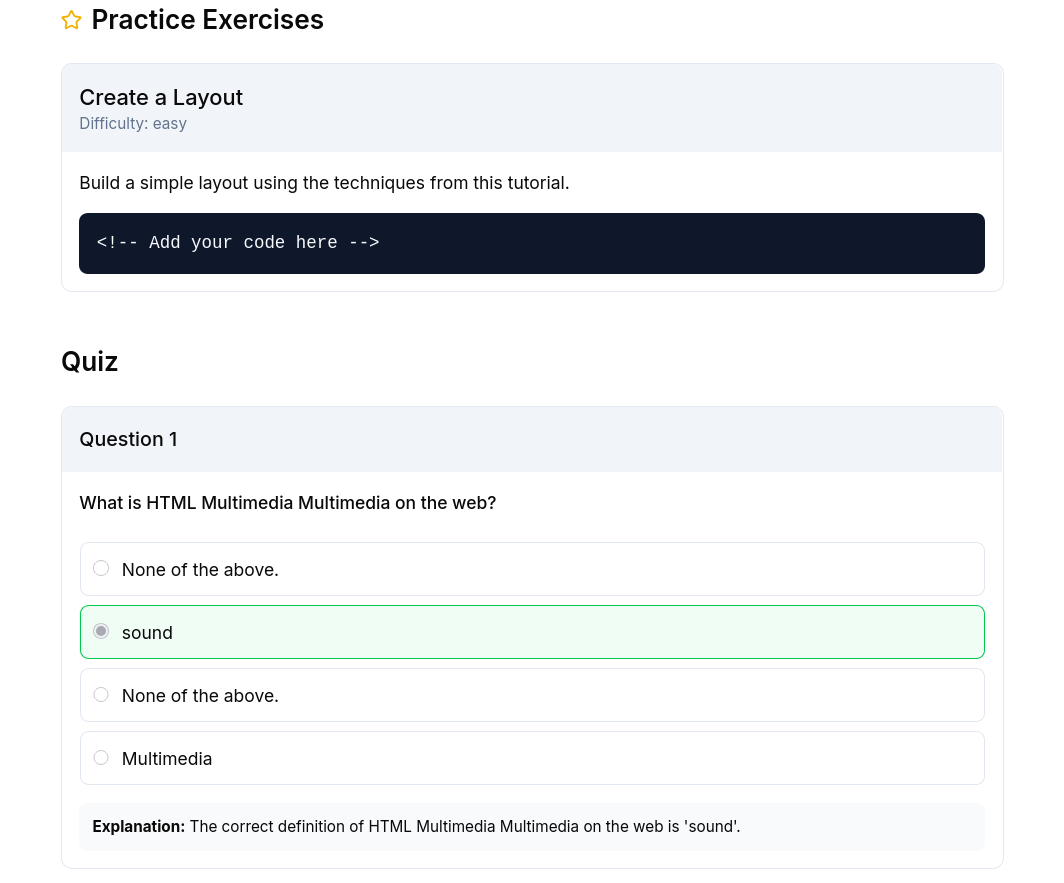
\includegraphics[width=\textwidth,height=4.5cm,keepaspectratio]{week_3_img/part2.png}
\end{center}
\end{columns}

\vspace{0.3cm}
\textbf{Certification:}
\begin{itemize}
    \item Badges and rewards to motivate learners
    \item Verifiable completion certificates
    \item Integration with professional networks
\end{itemize}
\end{frame}

% 5. Implementation Highlights (3 min)
\section{Implementation Highlights}

\begin{frame}
\frametitle{Technical Challenges}
\begin{itemize}
    \item \textbf{Content data processing}
    \begin{itemize}
        \item Difficulty automatically separating explanatory content from code
        \item Conventional approaches limited to 80\% accuracy
        \item Large volume of data to process (70+ courses)
    \end{itemize}
    \item \textbf{Code editor performance}
    \begin{itemize}
        \item Complex integration of Monaco Editor
        \item Secure execution of user code
        \item Optimization for mobile devices
    \end{itemize}
    \item \textbf{Rich and complex interfaces}
    \begin{itemize}
        \item Smooth animations without performance impact
        \item Dynamic UI component management
        \item Loading optimization
    \end{itemize}
\end{itemize}
\end{frame}

\begin{frame}
\frametitle{Implemented Solutions}
\begin{columns}
\column{0.48\textwidth}
\textbf{LLM processing pipeline:}
\begin{itemize}
    \item Parallel LLM models
    \item Asynchronous processing
    \item Intelligent segmentation
    \item Processing time reduction: 15h → 7-8h
    \item Accuracy near 100\%
\end{itemize}

\column{0.48\textwidth}
\textbf{Interactive code editor:}
\begin{itemize}
    \item Syntax highlighting (6+ languages)
    \item Real-time execution
    \item Customizable layouts
    \item Adaptable themes
    \item Full-screen mode
\end{itemize}
\end{columns}

\vspace{0.3cm}
\begin{center}
    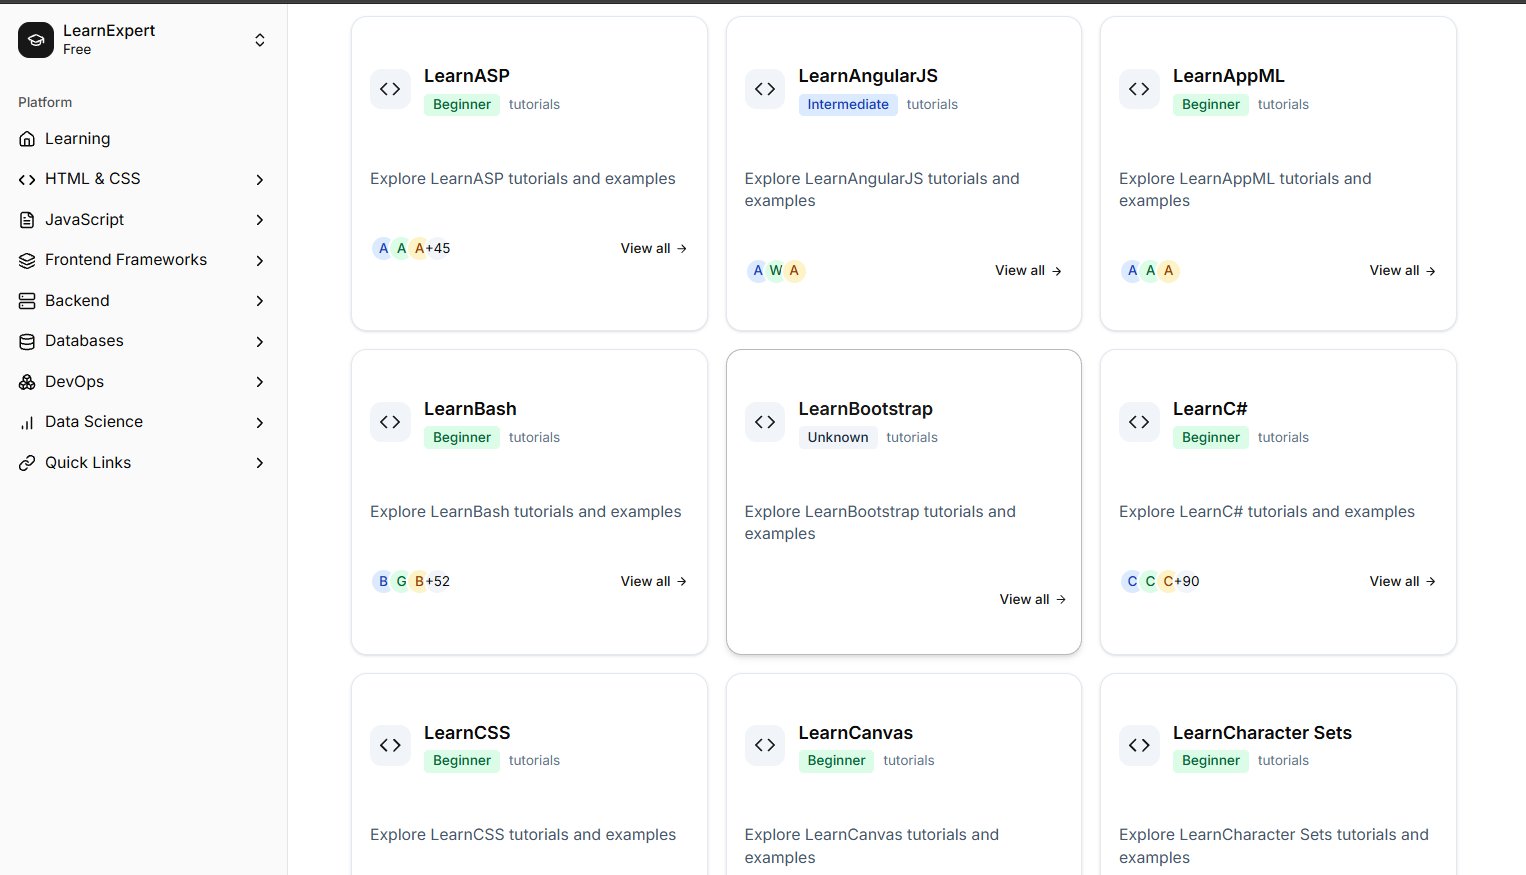
\includegraphics[width=0.6\textwidth,height=3.3cm,keepaspectratio]{week_3_img/Screenshot 2025-05-20 164411.png}
\end{center}
\end{frame}

\begin{frame}
\frametitle{Performance Optimizations}
\begin{itemize}
    \item \textbf{Frontend}
    \begin{itemize}
        \item Code splitting and lazy loading of components
        \item Automatic image optimization
        \item Intelligent resource preloading
        \item Selective caching
    \end{itemize}
    \item \textbf{Backend}
    \begin{itemize}
        \item Optimized database indexing
        \item Caching of frequent queries
        \item Load-balancing API Gateway
        \item Response compression
    \end{itemize}
    \item \textbf{Infrastructure}
    \begin{itemize}
        \item Vercel deployment for frontend
        \item Docker containerization for backend services
        \item Optimized Nginx configuration
    \end{itemize}
\end{itemize}
\end{frame}

% 6. Project Timeline (2 min)
\section{Project Timeline}

\begin{frame}
\frametitle{Development Timeline}
\begin{center}
    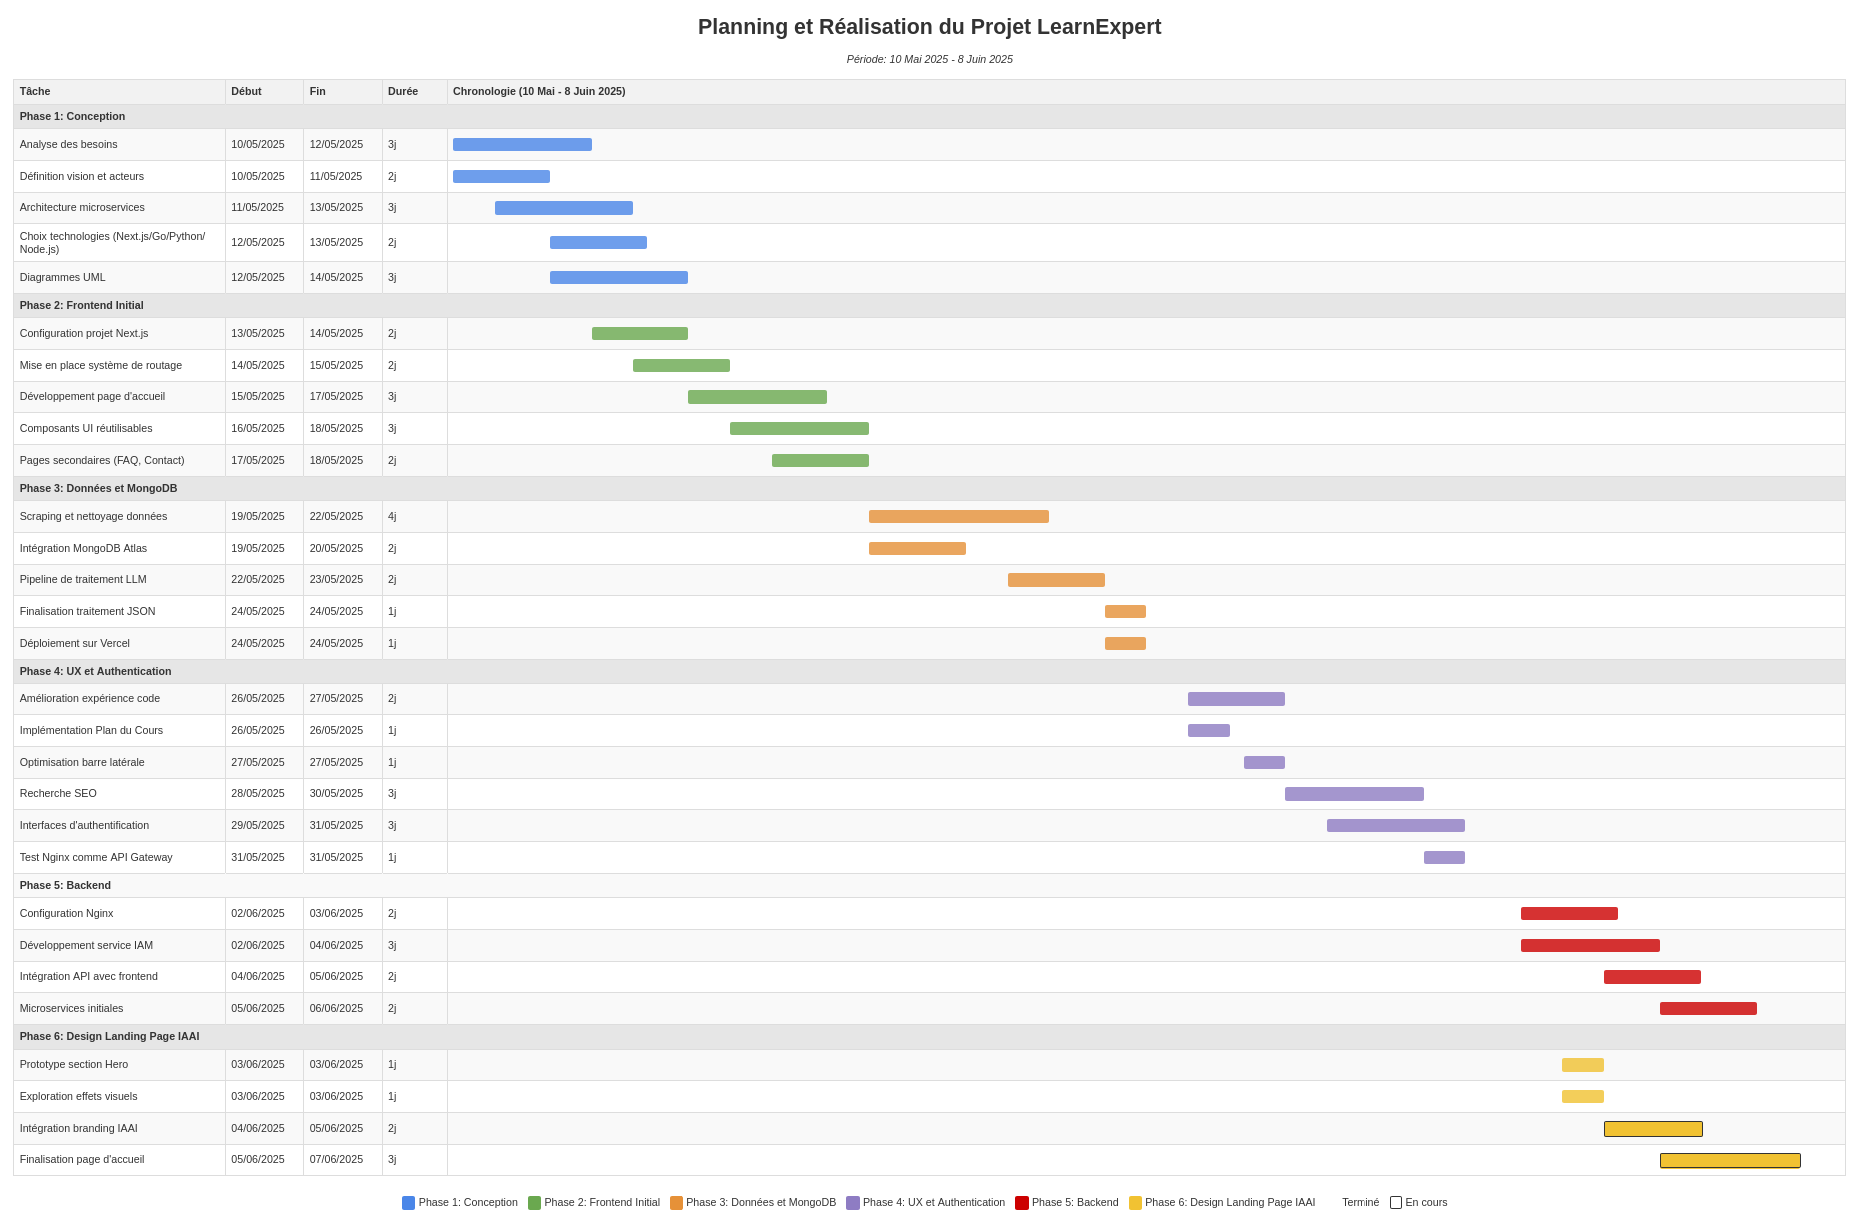
\includegraphics[width=0.95\textwidth,height=7cm,keepaspectratio]{Screenshot 2025-06-08 at 20-35-06 Planning du Projet LearnExpert - Diagramme de Gantt.png}
\end{center}
\end{frame}

\begin{frame}
\frametitle{Critical Path Analysis}
\begin{itemize}
    \item \textbf{Identified critical phases:}
    \begin{itemize}
        \item Initial design
        \item Main frontend development
        \item Secondary page implementation
        \item Essential backend services
    \end{itemize}
    \item \textbf{Effective parallelization:}
    \begin{itemize}
        \item UI development and routing system
        \item Backend and data processing
        \item Frontend design and integration
    \end{itemize}
    \item \textbf{Balanced distribution:} 4 weeks divided into logical phases
\end{itemize}
\end{frame}

% 7. Conclusion & Future Work (2 min)
\section{Conclusion and Future Work}

\begin{frame}
\frametitle{Project Results}
\begin{columns}
\column{0.5\textwidth}
\textbf{Main achievements:}
\begin{itemize}
    \item Functional microservices architecture
    \item Intuitive and responsive user interface
    \item Interactive code editor
    \item Optimized data processing pipeline
    \item Secure authentication system
\end{itemize}

\column{0.5\textwidth}
\textbf{Skills acquired:}
\begin{itemize}
    \item Next.js and React mastery
    \item Microservices architecture experience
    \item Advanced use of MongoDB and Supabase
    \item LLM model integration
    \item Agile development in real context
\end{itemize}
\end{columns}
\end{frame}

\begin{frame}
\frametitle{Future Perspectives}
\begin{itemize}
    \item \textbf{For IAAI:}
    \begin{itemize}
        \item Enhanced AI features for learning path personalization
        \item Advanced learner performance analytics
        \item Adaptive content generation
    \end{itemize}
    \item \textbf{Planned technical developments:}
    \begin{itemize}
        \item Native mobile application
        \item Third-party platform integration
        \item Multilingual expansion
        \item Collaborative features
    \end{itemize}
    \item \textbf{Next steps:}
    \begin{itemize}
        \item Beta version launch
        \item Large-scale user testing
        \item Continuous optimization based on feedback
    \end{itemize}
\end{itemize}
\end{frame}

\begin{frame}
\frametitle{Questions?}
\begin{center}
    \LARGE Thank you for your attention!\\
    \vspace{1cm}
    Questions?
\end{center}
\end{frame}

\end{document} 